\begin{table*}[t]
  \begin{minipage}[t]{0.54\textwidth}
    \centering
    \caption{Per-engine out-of-context synthesis, Nangate45 \SI{45}{\nano\meter},
             all constrained at a common period.
             Zero hold and zero electrical violations in every run.}
    \label{tab:synth}
    \label{fig:throughput_comparison}
    \setlength{\tabcolsep}{2.5pt}
    \renewcommand{\arraystretch}{1.15}
    \resizebox{\linewidth}{!}{%
    \begin{tabular}{|l|r|r|r|r|r|r|}
      \hline
      Engine & Elem./ & Area & $F_{\max}$ & Power & Throughput & Density \\
             & instr. & (\si{\micro\meter\squared}) & (\si{\mega\hertz}) & (\si{\milli\watt})
             & (\si{\giga\flop\per\second}) & (\si{\giga\flop\per\second\per\milli\meter\squared}) \\
      \hline
      \fpfour     & 16 & 13{,}442 & 414.9 & 246.0 & 13.28 & 988 \\
      \hline
      \mtwo       & 16 & 16{,}419 & 359.5 & 441.0 & 11.50 & 701 \\
      \hline
      \fpeight    &  8 & 23{,}881 & 288.3 & 193.0 &  4.61 & 193 \\
      \hline
      \insn{mxr4dot}  & 16 & 13{,}070 & 915.5 & 173.0 & 29.30 & \textbf{2{,}241} \\
      \hline
      \insn{mxfinal} & 16 & 11{,}149 & 441.0 & 148.0 & 14.11 & \textbf{1{,}266} \\
      \hline
    \end{tabular}%
    }
    \\[2pt]
    \begin{minipage}{\linewidth}
      \footnotesize
      \insn{mxr4dot} and \insn{mxfinal} are the two pipelined stages of the \fpfourres{} instruction pair (\S\ref{sec:arch-isa}). \insn{mxr4dot} performs scale-free reduction (29.30\,GFLOP/s, 173.0\,mW), while \insn{mxfinal} completes FP32 accumulation and rounding (14.11\,GFLOP/s, 148.0\,mW), bounding the pair's throughput at 14.11\,GFLOP/s.
    \end{minipage}
  \end{minipage}%
  \hfill
  \begin{minipage}[t]{0.43\textwidth}
    \centering
    \vspace*{10pt}
    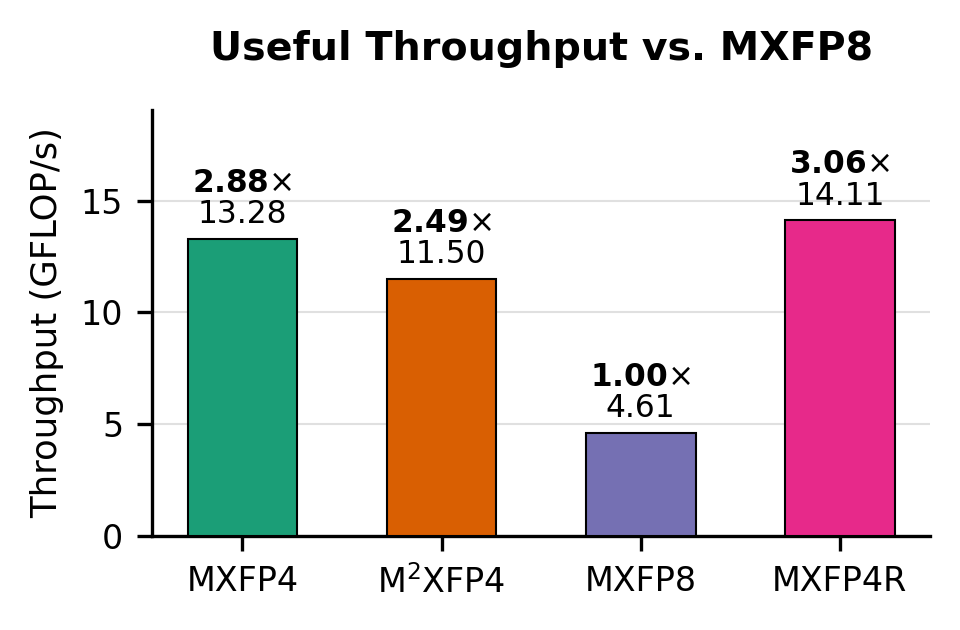
\includegraphics[width=\linewidth]{mxfp4r_throughput_comparison.png}
  \end{minipage}
\end{table*}
